%!TEX root = Main.tex
\documentclass[Main]{subfiles}

\begin{document}

\subsection{Class diagrams}
The class diagram for the server is described on Figure \ref{fig:serverClass}. 
Compared with Exercise 3, the Leader/follower pattern (\code{LF\_Event\_Handler}) inherits and point to the \code{Event\_handler} and uses the pool of threads, and \code{LF\_Thread\_Pool}.
The \code{Acceptor} is parameterized by a template, \code{SERVICE\_HANDLER} to be able to instantiate different kinds of service handlers.

\begin{figure}[hbtp]
\centering
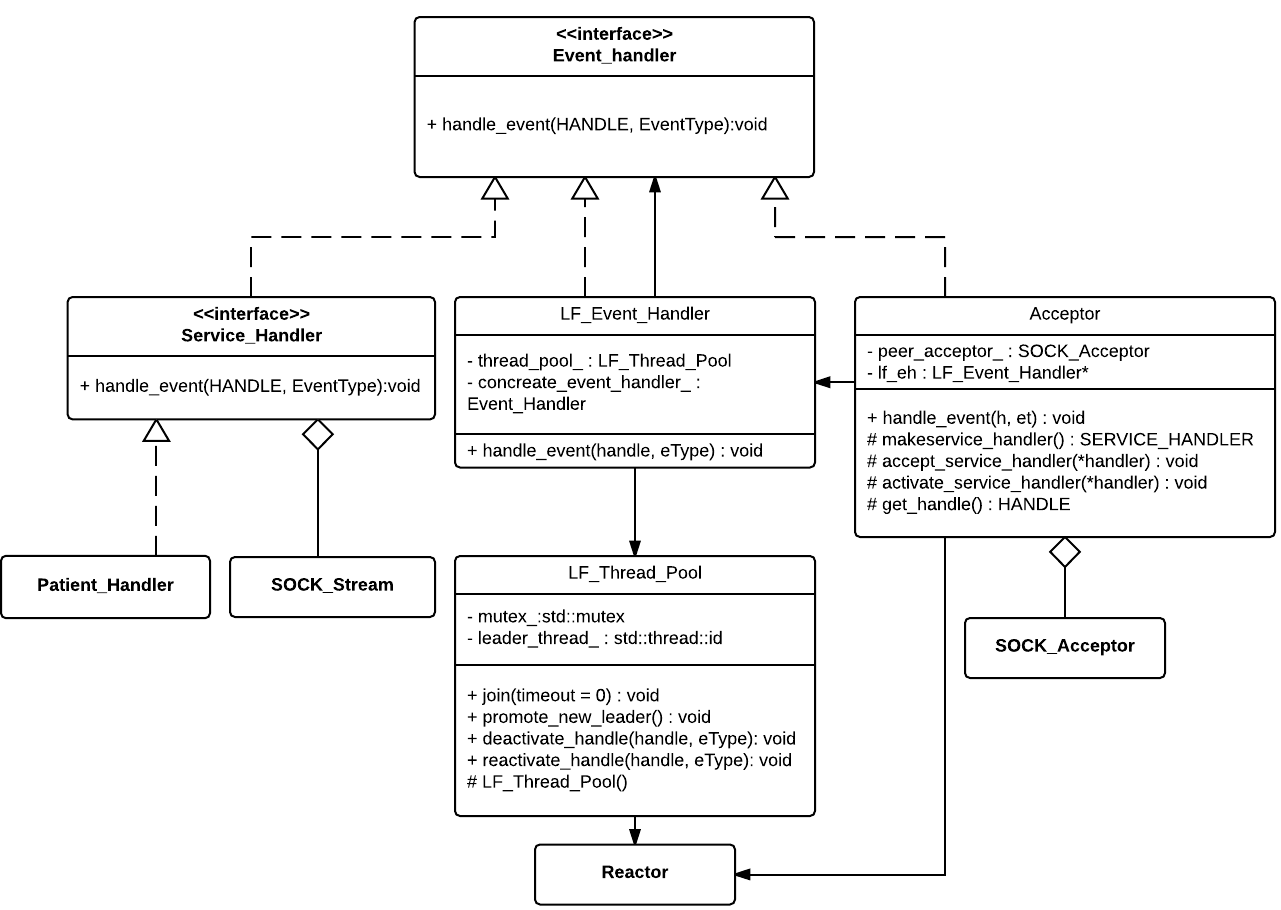
\includegraphics[width=1 \textwidth]{ServerDiagram2}
\caption{Class diagram for the server}
\label{fig:serverClass}
\end{figure}

\end{document}